\documentclass[journal = jacsat, manuscript = suppinfo]{achemso}

\usepackage[version = 4]{mhchem}
\usepackage{graphicx}
\usepackage{mwe}
\usepackage{gensymb}
\usepackage{titlesec}

% disable symbol next to email
\makeatletter
\def\acs@author@fnsymbol#1{}
\makeatother
% enable TOC
\SectionNumbersOn
% cool subsections
\titleformat{\subsection}[runin]{}{\textbf\thesubsection\quad}{0pt}{\textbf}[]

% macros
\newcommand{\h}{$^1$H}
\newcommand{\p}{$^{31}$P}
\newcommand{\cdcl}{\ce{CDCl3}}
\newcommand{\del}{$\delta = $}
\newcommand{\nh}{\ce{NH3}}
\newcommand{\wavenum}{cm$^{-1}$}
\newcommand{\nicl}{\ce{NiCl2 $\cdot$ 6H2O}}
\newcommand{\ninh}{\ce{[Ni(NH3)6]Cl2}}
\newcommand{\nicp}{\ce{Ni(Cp)2}}
\newcommand{\nutilde}{$\widetilde\nu = $}

\title{Synthesis of nickelocene via ligand substitution of \nicl}

\author{David Qiu}
\affiliation{Department of Chemistry, University of Illinois at
Urbana-Champaign, 505 S Matthews Avenue, Urbana, IL, 61801}
\email{davidlq2@illinois.edu}

\begin{document}

\tableofcontents

\section{General Considerations}

Throughout the experiment, a 60 MHz Nanalysis NMReady-60PRO tabletop NMR
instrument was used to record all \h\ NMR spectra at room temperature. NMR
spectrum was sourced from a fellow classmate. IR spectra were taken on a Perkin
Elmer Spectrum Two FTIR spectrometer. The experiment was performed according to
Girolami et al.\cite{textbook}

Diethyl ether was sourced from Fischer Chemical. Ammonium hydroxide
(28.0\%--30.0\% \nh) was sourced from Macron Fine Chemicals. \nicl\ and NaCp
(2.4 M in THF) was sourced from Sigma-Aldrich. Ethanol and THF sourced directly
from the University of Urbana-Champaign Chemistry department.

\section{Experimental}

\subsection{\ninh\ synthesis} \nicl\ (8 g, 34 mmol)  was mixed with 20 mL DI
water in a flask. While stirring, 30 mL of concentrated ammonium hydroxide
(28.0\%\textendash 30.0\% \nh) was poured in, forming a cloudy purple mixture.
This solution was cooled in an ice bath, and 80 mL of ethanol was added. The
\ninh\ precipitate was filtered through a coarse glass frit, and was washed with
ethanol and diethyl ether. The \ninh\ was then dried, yielding a percent yield
of 85.5\% (6.74 g total, 7.88 g expected).

\subsection{\nicp\ synthesis} \ninh\ (1.2 g, 5 mmol) and a stir bar was added
to a three-necked round-bottom flask placed in an ice bath. A gas inlet valve,
glass stopper, and rubber septum were attached, and the flask was filled with
\ce{N2} on a Schlenk line. 20 mL of THF was injected, and 5 mL of NaCp was added
drop-wise. This was allowed to react for 1 hour, during which the solution
turned a dark brown. The reaction was quenched with 1 mL of ethanol. Residual
solvent was removed via the Schlenk line. The rubber stopper was quickly
replaced with a glass stopper, and all joints were re-greased.

\subsection{\nicp\ sublimation and analysis} A cold finger was quickly fitted to
the central neck of the \nicp\ flask, and the flask was placed under a static
vacuum. The flask was then heated via a heating mantle between 80--120 \degree C
(40 V on a Variac), and green crystals gradually formed on the cold finger over
an hour.  The flask was then refilled with \ce{N2}, and the sublimed \nicp\
crystals were then weighed, yielding a percent yield of 10.6\% (0.10 g total,
0.94 g expected).  \h\ NMR and IR spectrum were collected.

\h\ NMR (60 MHz, \cdcl): 7.21 ppm (\ce{CHCl3}, s), 2.20 ppm (acetone, s), 1.35
ppm (H grease, m), 0.12 ppm (unidentified impurity). Impurities were identified
according to a table of trace impurities.\cite{nmrtable} The \nicp\ product
shift was not observed in the \h\ NMR. This interpretation is in good agreement
with the literature value of the \h\ NMR shift of nickelocene (254.8 ppm).\cite{ni-book}

IR: \nutilde\ 2963 \wavenum (C-H stretch), \nutilde\ 1422 \wavenum (asymmetric
aromatic C-C stretch), \nutilde\ 1259 \wavenum (C-H bend/rock). This is in good
agreement with the literature nickelocene IR spectra, which cite additional
vibrational modes of the cyclopentadienyl ligand in the fingerprint
region.\cite{ni-book, ni-paper}

\section{\h\ NMR Spectrum}

\begin{figure}[H]
	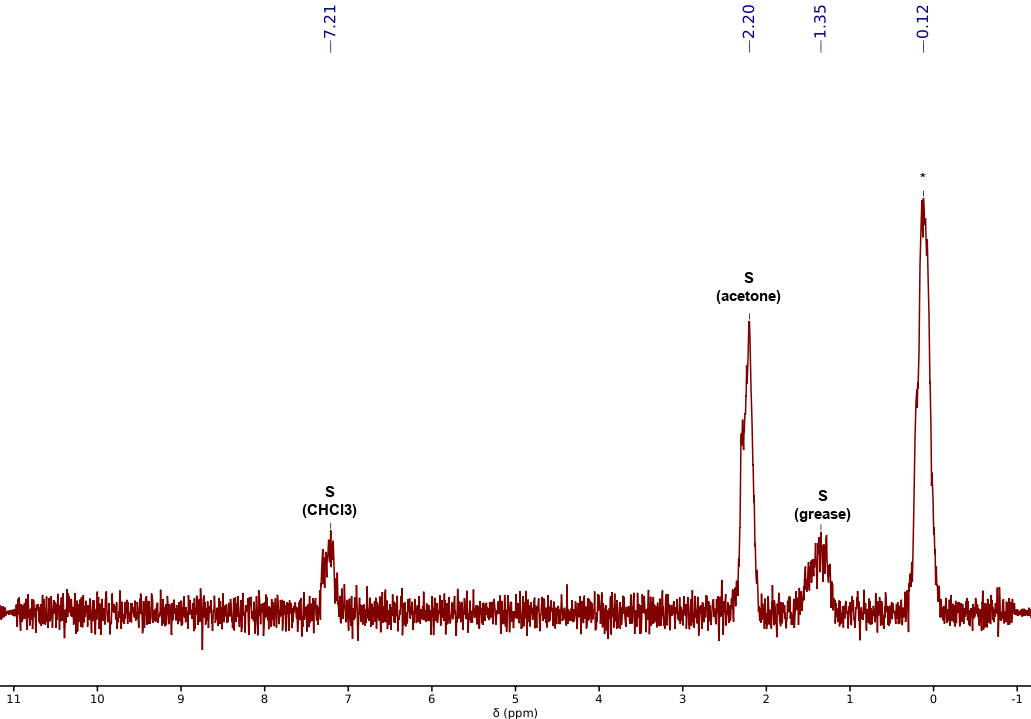
\includegraphics[width=\textwidth]{figures/nickelocene_hnmr.png}
	\caption{Provided \h\ NMR spectrum of \nicp, following baseline and
	phase correction.``S" denotes residual non-deuterated organic solvents,
	and ``*" denotes an unidentified impurity.}
\end{figure}


\section{IR Spectrum}

\begin{figure}[H]
	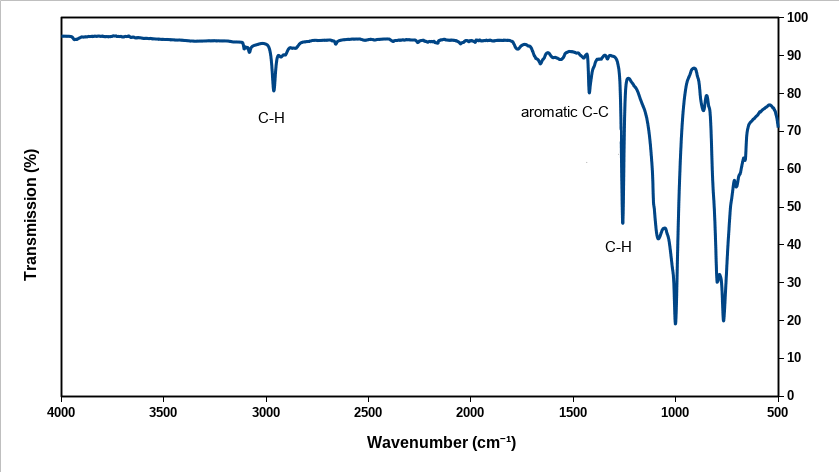
\includegraphics[width=\textwidth]{figures/nickelocene_ir.png}
	\caption{IR spectrum of \nicp, with corresponding assignments.}
\end{figure}

\bibliography{lab_4.bib}

\end{document}
